\documentclass[a4paper]{article}
\usepackage[top=1in, bottom=1.25in, left=1.25in, right=1.25in]{geometry}


\usepackage{amsmath}
\usepackage{amssymb}
\usepackage{graphicx}
\usepackage[utf8]{inputenc}
 
\usepackage{amsthm}
\usepackage{enumitem}   
\usepackage{listings}

\lstset{
  breaklines=true,
  numbers=left,
  language=Python
}

\begin{document}

%% Title, authors and addresses

\title{Brain Inspired Computing - Problem Set 4}

\author{Sven Bordukat, Paul Meehan}

\date{\today}

\maketitle


\section*{Exercise 3}
\begin{itemize}
    \item [a)] Through empirical estimation following values are found:\\
    \linebreak
    \begin{tabular}[h]{ll}
        $v_{rest}$&-$70mV$\\
        $w_e$&$0.0035\mu S$\\
        $w_i$&$0.048 \mu S$\\
        $\tau_m$&$9.9 ms$\\
        $\tau_{syn}^e$&$2.9ms$\\
        $\tau_{syn}^i$&$5.2ms$\\
    \end{tabular}
\item [b)] Shown here are the simulation with the noise removed, as well as
the original data; the noise was removed from the simulation as it was hard to
plot and discern the different noisy lines.
\end{itemize}
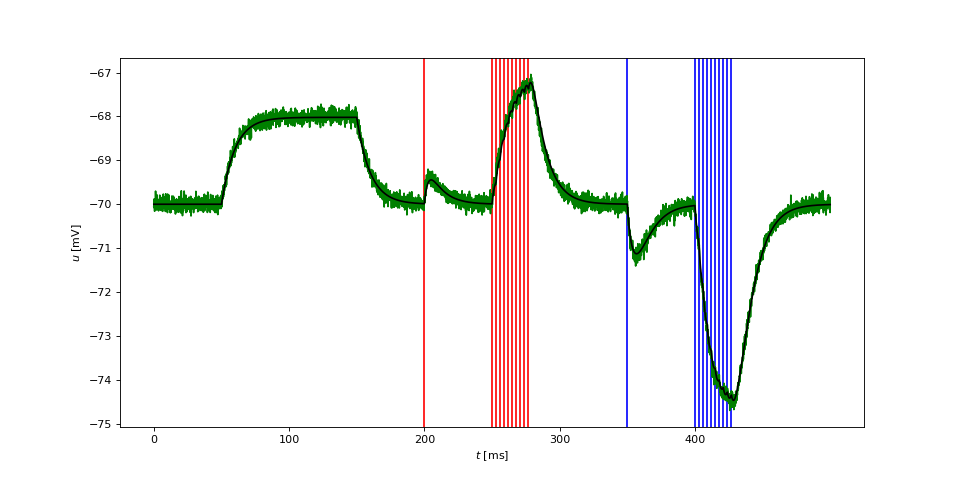
\includegraphics[width=\textwidth]{3.png}
\end{document}
